\newcommand{\lastversion}{0.1.0}%versione del documento
\newcommand{\doctitle}{Glossario}%nome documento
\newcommand{\info}{\doctitle\ v\lastversion}
\documentclass[11pt,a4paper]{article}
\usepackage[a4paper,portrait,top=3.5cm,bottom=3.5cm,left=3cm,right=3cm,bindingoffset=5mm]{geometry}


\usepackage[italian]{babel}
\usepackage{ucs} %unicode sistema gli accenti
\usepackage[utf8x]{inputenc} %unicode sistema gli accenti
\usepackage{fancyhdr}
\usepackage{subfigure} % per figure affiancate
\usepackage{hyperref}
\usepackage{float} % per far bene le figures
\usepackage{indentfirst}
\usepackage{longtable}
\usepackage{color}
\usepackage{colortbl}
\usepackage{rotating}
\usepackage[table]{xcolor}
\usepackage{wrapfig}
\usepackage{array}
\usepackage{eurosym}
\usepackage{graphicx}
\usepackage{breakurl}
\usepackage{lastpage} % total page count
\usepackage{chngpage}
\usepackage{amsfonts}
\usepackage{listings}
\usepackage{bookmark} % custom bookmarks

%\graphicspath{{./Pics}} % cartella di salvataggio immagini

% Per l'indice analitico
%\usepackage{makeidx}
%\makeindex

%pagestyle{fancy}
%\renewcommand{\chaptermark}[1]{\markboth{\thechapter.\ #1}{}}
%\renewcommand{\sectionmark}[1]{\markright{\thesection.\ \ #1}{}}
%\fancyhead{}
%comandi dell header
%\fancyhead[EL]{\slshape \leftmark}
%\fancyhead[OR]{\slshape \rightmark}
%\fancyfoot[EC,OC]{\slshape \thepage}

\pagestyle{fancy}
%\newcommand{\license}{\href{http://creativecommons.org/licenses/by/3.0/}{Some rights reserved}}
\newcommand{\groupname}{Sirius - Sequenziatore}

\newcommand{\subscript}[1]{\raisebox{-0.6ex}{\scriptsize #1}}
%\newcommand{\subscript}[1]{\ensuremath{_{\textrm{#1}}}}
%\renewcommand{\sectionmark}[1]{\markright{\thesection.\ #1}}
%\lhead{\nouppercase{\rightmark}}
%\rhead{\nouppercase{\leftmark}}
%\renewcommand{\chaptermark}[1]{\markboth{\thechapter.\ #1}{}}


\fancypagestyle{plain}{%
	\chead{}
	\lfoot{\info}
	\cfoot{}
	\rfoot{\thepage\ / \pageref{LastPage}}
	\renewcommand{\headrulewidth}{0.3pt}
	\renewcommand{\footrulewidth}{0.3pt}
}
	\lhead{\setlength{\unitlength}{1mm}
        \begin{picture}(0,0)
                \put(5,0){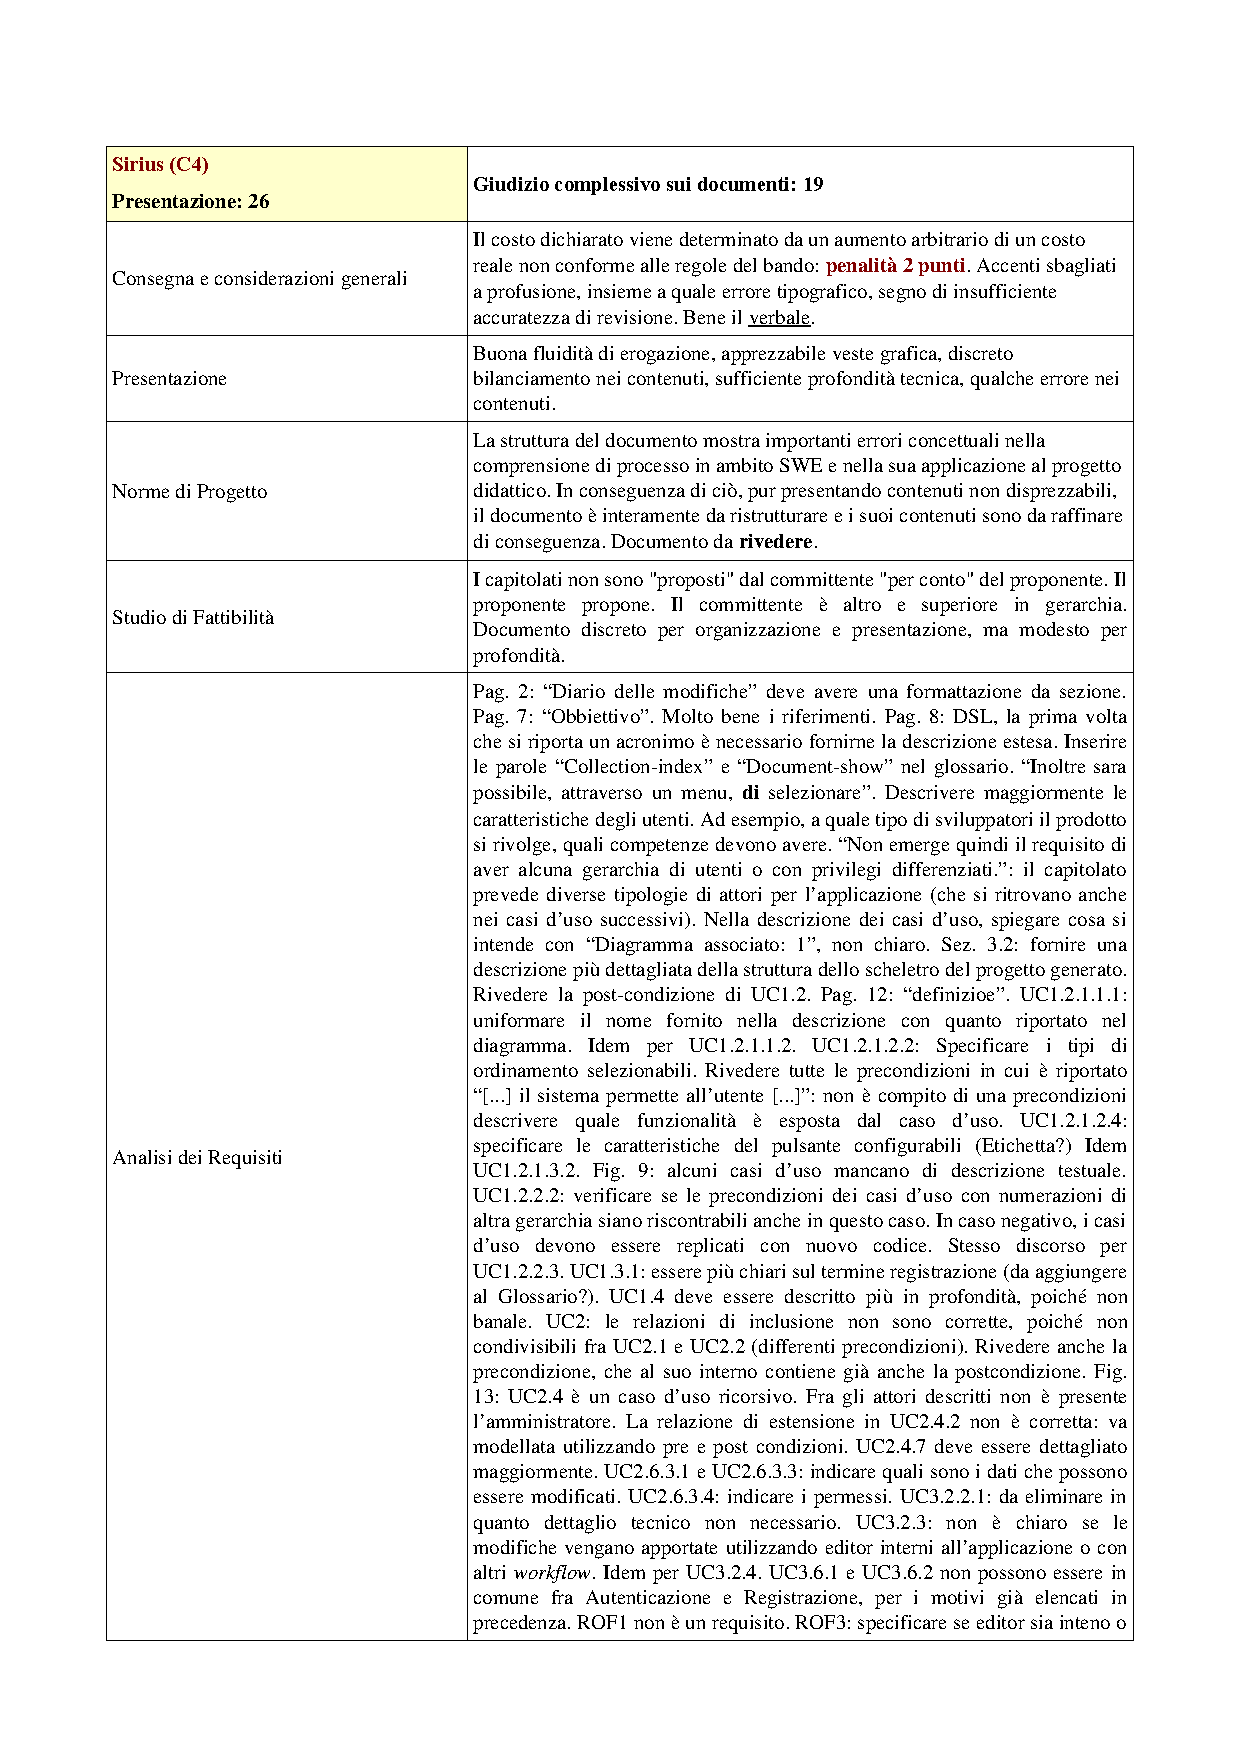
\includegraphics[scale=0.001]{img/Sirius.png}}
        \end{picture}}
	\rhead{\groupname}
	\chead{}
	\lfoot{\info}
	\cfoot{}
%	\rfoot{\thepage}
	\rfoot{\thepage\ / \pageref{LastPage}}
	\renewcommand{\headrulewidth}{0.3pt}
	\renewcommand{\footrulewidth}{0.3pt}
\linespread{1.2}	% valore interlinea


\fancypagestyle{romano}{
	\lhead{\setlength{\unitlength}{1mm}
        \begin{picture}(0,0)
                \put(5,0){
\includegraphics[scale=0.03]{../modello/img/sirius.png}}
        \end{picture}}
	\chead{}
	\rhead{\groupname}
	\lfoot{\info}
	\cfoot{}
	\rfoot{\thepage}
	\renewcommand{\headrulewidth}{0.3pt}
	\renewcommand{\footrulewidth}{0.3pt}
}



\hypersetup{
    colorlinks=true,linkcolor=[rgb]{0.11,0.55,0.83
    },          % colore link interni
    urlcolor=cyan           %colore link esterni
}
\definecolor{err}{rgb}{0.9,0.1,0.1}
\definecolor{rt}{rgb}{0.1,0.6,0.8}
\definecolor{grey}{rgb}{0.4,0.3,0.4}
\definecolor{mycolor}{rgb}{0.67,1,0.18}

\bibliographystyle{plain_ita}%bibliografia stile italiano

\pagenumbering{Roman}
\setlength\parindent{0pt} % sempre senza indentatura
% fine layout% layout
\begin{document}
% Prima pagina di opgni documento
\begin{titlepage}
 \begin{center}
     
\includegraphics[width=11cm]{../modello/img/sirius}\\
     \vspace{1em}
     {\LARGE \textsc{Sirius}}\\
     \vspace{2em} \hrule \vspace{2em}
     {\Large \textsc{Sequenziatore}}\\
     \vspace{8em}
     {\LARGE \LARGE \LARGE \textbf{\doctitle}}\\
     \vspace{2em}
     {\LARGE \LARGE \LARGE \textbf{Versione \lastversion }}\\
     \vspace{4em}
 \end{center}


\vskip 1.8cm
\begin{center}
\textit{Ingegneria Del Software AA 2013-2014}
\end{center}

\end{titlepage}


%pagina del titolo
\thispagestyle{romano}
\noindent\begin{Large}\textbf{Informazioni documento}\end{Large}\\
\begin{center}
\begin{tabular}{ll}
\hline\\
Titolo documento: & Analisi dei requisiti\\
Data creazione: & 1 Febbraio 2014\\
Versione attuale: & \lastversion\\
Utilizzo: & Esterno\\
Nome file:& \AnalisiDeiRequisiti{}\\
Redazione: & Botter Marco\\
& Giachin Vanni\\
& Marcomin Gabriele\\
Verifica: & Seresin Davide\\
Approvazione: & Quaglio Davide\\
Distribuito da:& Sirius\\
Destinato a: & Prof. Vardanega Tullio\\
			 & Prof. Cardin Riccardo\\
			 & Zucchetti S.p.A.
\end{tabular}
\end{center}
\vskip 1.5cm
%\noindent {\begin{LARGE}\textbf{Sommario}\end{LARGE}}\\
\noindent\begin{Large}\textbf{Sommario}\end{Large}\\

\noindent Risultato dello studio di fattibilità della ditta Sirius per il capitolato C04 Seq\\
\newpage
\pagestyle{romano}
\noindent\begin{Large}\textbf{Diario delle modifiche}\end{Large}\\
\\
%Inserire in testa ogni nuova versione\\
\begin{small}
\begin{tabular}{|c|p{1.8cm}|p{2.8cm}|p{2.8cm}|p{3.5cm}|}
\hline
Versione & Data & Autore & Ruolo & Descrizione \\
\hline
\hline
1.0.0 & 2014-03-05 & 
\textit{Quaglio Davide} &
\textit{Responsabile} &  Approvazione del documento\\
\hline
0.1.0 & 2014-02-13 & 
\textit{Botter Marco} &
\textit{Verificatore} &  Verifica del documento\\
\hline
0.0.2 & 2014-02-11 & 
\textit{Seresin Davide} &
\textit{Analista} &  Aggiunte e modifiche\\
\hline
0.0.1 & 2014-02-09 & 
\textit{Santangelo Davide} &
\textit{Analista} &  Creato lo scheletro del documento\\
\hline
\end{tabular}\\
\end{small}


\newpage
\pagestyle{romano}

\tableofcontents %sommario
\pagestyle{romano}



\newpage
\pagestyle{plain}
\pagenumbering{arabic}%numeri di pagina arabi
<<<<<<< HEAD:Glossario/Glossario.tex

\section{Introduzione}

\subsection{Scopo del documento}
Il documento definisce le norme, convenzioni e formalismi  che ciascun membro del gruppo \gruppo{} deve adottare durante l'intera produzione del software \progetto{}.
In particolare tali norme regolamentano i seguenti aspetti:

\begin{itemize}
\item Organizzazione tra i membri del gruppo;
\item Stili e convenzioni nella redazione dei documenti;
\item Metodi operativi e convenzioni nelle fasi di progetto;
\item Ambiente di lavoro.
\end{itemize}

\subsection{Glossario}
Al fine di facilitare la comprensione dei documenti, i termini tecnici, di dominio e gli acronimi, sono definiti in dettaglio nel documento GLOSSARIO.\\
Tali termini sono contrassegnati dal simbolo \ped{$\vert$G$\vert$} che li segue.
\newpage

\section{Definizioni}

=======
\section{Introduzione}

\subsection{Scopo del documento}
Il documento definisce le norme, convenzioni e formalismi  che ciascun membro del gruppo \gruppo{} deve adottare durante l'intera produzione del software \progetto{}.
In particolare tali norme regolamentano i seguenti aspetti:

\begin{itemize}
\item Organizzazione tra i membri del gruppo;
\item Stili e convenzioni nella redazione dei documenti;
\item Metodi operativi e convenzioni nelle fasi di progetto;
\item Ambiente di lavoro.
\end{itemize}

\subsection{Glossario}
Al fine di facilitare la comprensione dei documenti, i termini tecnici, di dominio e gli acronimi, sono definiti in dettaglio nel documento GLOSSARIO.\\
Tali termini sono contrassegnati dal simbolo \ped{$\vert$G$\vert$} che li segue.
\section{Descrizione generale}
\subsection{Prospettive del prodotto}
\subsection{Funzionalità del prodotto}
\subsection{Caratteristiche degli utenti}
\subsection{Vincoli generali}
\section{Casi d'uso}

%\section{Requisiti}
Le convenzioni utilizzate per l'identificazione e la definizione dei requisiti sono riportate nel documento \NormeDiProgetto{}. 
\subsection{Requisiti funzionali}
\subsubsection{Ambito utente}
\LTXtable{\textwidth}{RequisitiUtente.tex}
\subsubsection{Ambito amministratore}
\LTXtable{\textwidth}{RequisitiAmministratore.tex}
\subsection{Requisiti di qualità}
\LTXtable{\textwidth}{RequisitiQualita.tex}
\subsection{Requisiti di vincolo}
\LTXtable{\textwidth}{RequisitiVincolo.tex}
>>>>>>> origin/marcomin:AnalisiDeiRequisiti/AnalisiDeiRequisiti.tex

\end{document}